%! Author = denis
%! Date = 20/08/2026

\begin{frame}{Latch SR (Set-Reset)}
    
    \begin{columns}[T]

        \begin{column}{0.60\textwidth}
            \centering
            \href{https://www.falstad.com/circuit/e-nandff.html?}{
            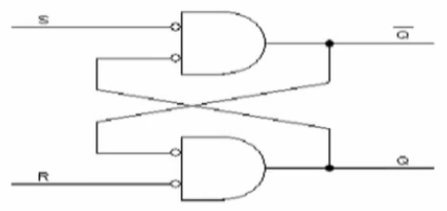
\includegraphics[
                width=0.8\textwidth
            ]{images/flip_flop_sr_1.png}
            }
            \vspace{0.2cm}

            {\scriptsize Latch SR - NAND}
        \end{column}

        \begin{column}{0.60\textwidth}
            \centering

            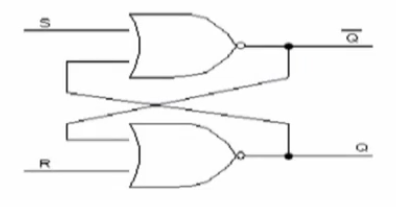
\includegraphics[
                width=0.8\textwidth
            ]{images/flip_flop_sr_2.png}

            \vspace{0.2cm}

            {\scriptsize Latch SR - NOR}
        \end{column}
    \end{columns}
    \vspace{1cm}
    \begin{itemize}
        \item Latch SR com portas NAND: Ativas em nível baixo.
        \item Latch ST com portas NOR: Ativas em nível alto.
    \end{itemize}
\end{frame}
